\documentclass[a4paper,utf8]{article}
\usepackage[heading,fancyhdr]{ctex}
\usepackage{amsmath,amssymb,geometry,lastpage,ulem}
\usepackage{array,tabularx,tabulary,mhchem,xspace}
\usepackage{floatrow,subfig,multirow,bigstrut}
\usepackage{siunitx,booktabs,longtable,graphicx,xfrac,nameref}
\lineskiplimit=1pt
\lineskip=3pt
\geometry{
    top=25.4mm, 
    left=25mm, 
    right=25mm, 
    bottom=25mm,
    headsep=5.9mm,
}
\ctexset{
    section = {format+=\raggedright}
}
\newcommand{\fgref}[1]{图~\ref{#1}\xspace}
\newcommand{\seqref}[1]{式~(\ref{#1})}
\newcommand{\expinfo}[7][无]{
    {\zihao{-3}\bfseries\songti
    实验名称:\uline{\hfill\mbox{#2}\hfill} \\[2.9mm]
    学\quad 号:\uline{\makebox[25mm]{#3}}\hfill
    姓\quad 名:\uline{\makebox[25mm]{#4}}\hfill
    班\quad 级:\uline{\makebox[25mm]{#5}} \\[2.9mm]
    合作者:\uline{\makebox[25mm]{#1}} \hfill
    桌\quad 号:\uline{\makebox[25mm]{#6}}\hfill\makebox[25mm+4em]{}\\[2.9mm]
    实验日期:\uline{\makebox[30mm]{#7}}\hfill\mbox{} \\[58.7mm]
    }
}
\newcommand{\pointingbox}{
    {\zihao{4}\bfseries\songti%
    实验考核\\[3mm]
    \extrarowheight=3mm
    \begin{tabularx}{150mm}{|X|X|X|X|X|}\hline
        \hfil 项目 \hfil  & \hfil 实验预习 \hfil & \hfil 实验过程 \hfil & \hfil 分析与讨论 \hfil & \hfil 总评 \hfil \\[3mm] \hline
        \hfil 评价 \hfil &  &  &  &  \\[3mm] \hline
    \end{tabularx}
    }
}
\newcommand{\derivative}[2]{\frac{\mathrm{d} #1}{\mathrm{d} #2}}
\newcommand{\thinking}[2]{\textbf{#1}\\
答:\begin{minipage}[t]{0.85\textwidth}
    #2
\end{minipage}}
\pagestyle{fancy}
\fancyhf{} \fancyhead[C]{电路基础实验} \fancyfoot[C]{\thepage~/~\pageref{LastPage}}
\newcounter{Rownumber}
\newcommand*{\Rown}{\stepcounter{Rownumber}\theRownumber}
\newcommand*{\resetRown}{\setcounter{Rownumber}{0}}
\newcommand{\qrange}[3]{\qtyrange[range-phrase = \text{$\sim$},range-units =single]{#1}{#2}{#3}}
\floatsetup[table]{capposition=top}
\newcolumntype{C}{>{\hfil}X<{\hfil}}
\renewcommand{\Nameref}[1]{\textbf{\ref{#1}~\nameref{#1}}} %导入导言

\begin{document}
\begin{center}
    {\mbox{}\\[7em]\zihao{2}\bfseries\songti%
    电路基础实验报告}\\[34mm]
    \expinfo[张泽钒]{一阶电路动态过程的研究}{22301077}{张蕴东}{22 高分子}{35}{2024.6.4}
\end{center}
\newpage

\section{实验目的}
\begin{enumerate}
    \item 研究一阶电路的零输入响应,零状态响应及全响应的基本规律和特点。
    \item 学习一阶电路时间常数 $\tau$ 的测量方法。
    \item 熟悉微分和积分电路结构,加深对构成微分和积分电路必要条件的理解。
    \item 熟悉示波器的使用方法。
\end{enumerate}

\section{实验原理}%简单描述,含必要的公式和附图;
\begin{itemize}
    \item 含有 L、C 元件的电路称动态电路。描述动态电路的方程是微分方程,由给定的初始条件可求得电路的响应。对线性电路其响应可分为零状态响应、零输入响应及全响应。初始状态为零,仅激励引起的响应叫零状态响应;激励为零,由初始条件引起的响应叫零输入响应;同时同激励和初始条件引起的响应叫全响应。电路中只含有一个电感或电容元件时称为一阶电路。
    \item 一阶电路的零输入响应总是按指数规律衰减,零状态响应总是按指数规律递增或递减,衰减和递增速率的快慢,决定于电路本身参数所确定的时间常数$\tau$。在 RC 电路中,$\tau=RC$;在 RC 电路中,$\tau=L/R$。
    \item 动态电路的过渡过程是短暂的单次变化过程,在瞬间发生又很快消失,所以观察这一过程是有困难的,常用方法是用方波仪记录其过程。在实验室中,根据电路时间常数τ的大小不同分别采用不同的实验方法。当$\tau$较大时(数秒),一般采用卡秒表的方法,即在“换路”的同时,既观测电压(或电流)的数值,又启动秒表记录时间,从而可以记录下电压(或电流)随时间变化的规律。当τ较小时,一般采用示波器观测。为了便于观测,必须使单次过渡过程重复出现。可以用方波的前沿代替单次接通直流电源,这样,在方波的每一个前沿和后沿,都出现一次过渡过程。
    \item 微分电路和积分电路是脉冲数字电路中最常见的波形变换电路。如果输入是方波信号,对于微分电路,当电路时间常数 $\tau$ 远远小于方波的脉冲宽度 $T_p$(20 倍以上)时,电路输出与输入近似呈微分关系,即将方波变换成正负极性的尖脉冲;对于积分电路,如果电路时间常数 $\tau$ 远远大于方波的脉冲宽度 $T_p$(20 倍以上),电路输出与输入近似呈积分关系,即将方波变换成三角波。
\end{itemize}

\section{实验仪表}
    实验电路见电路原理实验箱《一阶电路动态过程的研究》单元,R1=3\unit{\kilo\ohm}、R2=5.1\unit{\kilo\ohm}、\linebreak R3=5.1\unit{\kilo\ohm} 、R4= 2.4\unit{\kilo\ohm}、C1= 10\unit{\uF}、C2= 0.1\unit{\uF}、L1= 100\unit{\mH}、L2= 100\unit{\mH}。在这个单元上,可以做 RC 微分、RC 积分、RL 微分、RL 积分。
    
\section{实验内容与结果}
    \subsection{微分电路}
        \subsubsection{RC微分电路}
            RC 微分电路如图~\ref{fig:1a} 所示,调节方波仪输出频率,使方波脉冲宽度满足微分电路的必要条件,将 R2、R4分别接入,观察微分电路输出有何不同,并将波形画在附表中。
        \subsubsection{RL微分电路}
            RL 微分电路如图~\ref{fig:1b} 所示,调节方波仪输出频率,使方波脉冲宽度满足微分电路的必要条件,将 R1、R3分别接入,观察微分电路输出有何不同,并将波形画在附表中。
    \subsection{积分电路}
        \subsubsection{RC积分电路}
            RC 积分电路如图~\ref{fig:4a} 所示,调节方波仪输出频率,使方波脉冲宽度满足微分电路的必要条件,将 R1、R3分别接入,观察微分电路输出有何不同,并将波形画在附表中。
        \subsubsection{RL积分电路}
            RL 微分电路如图~\ref{fig:4b} 所示,调节方波仪输出频率,使方波脉冲宽度满足微分电路的必要条件,将 R2、R4分别接入,观察微分电路输出有何不同,并将波形画在附表中。
    \newpage

    \subsection{实验结果}
        如图所示:\par
        \begin{figure}[!ht]
            \subfloat[RC微分电路图\label{fig:1a}]{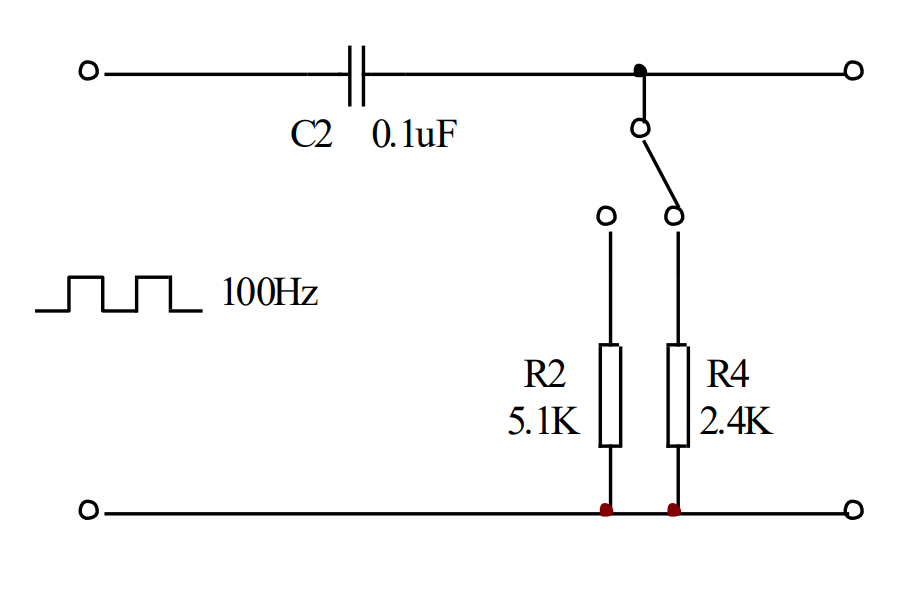
\includegraphics[width=0.35\textwidth]{1a.png}}\hspace{6mm}
            \subfloat[RL微分电路图\label{fig:1b}]{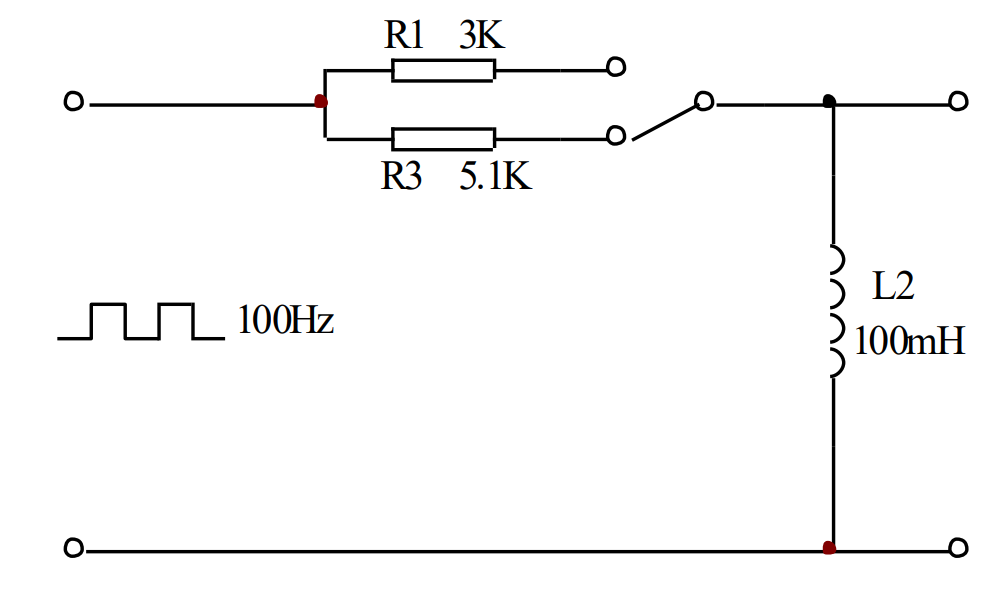
\includegraphics[width=0.35\textwidth]{1b.png}}\\
            \subfloat[电路波形\label{fig:2}]{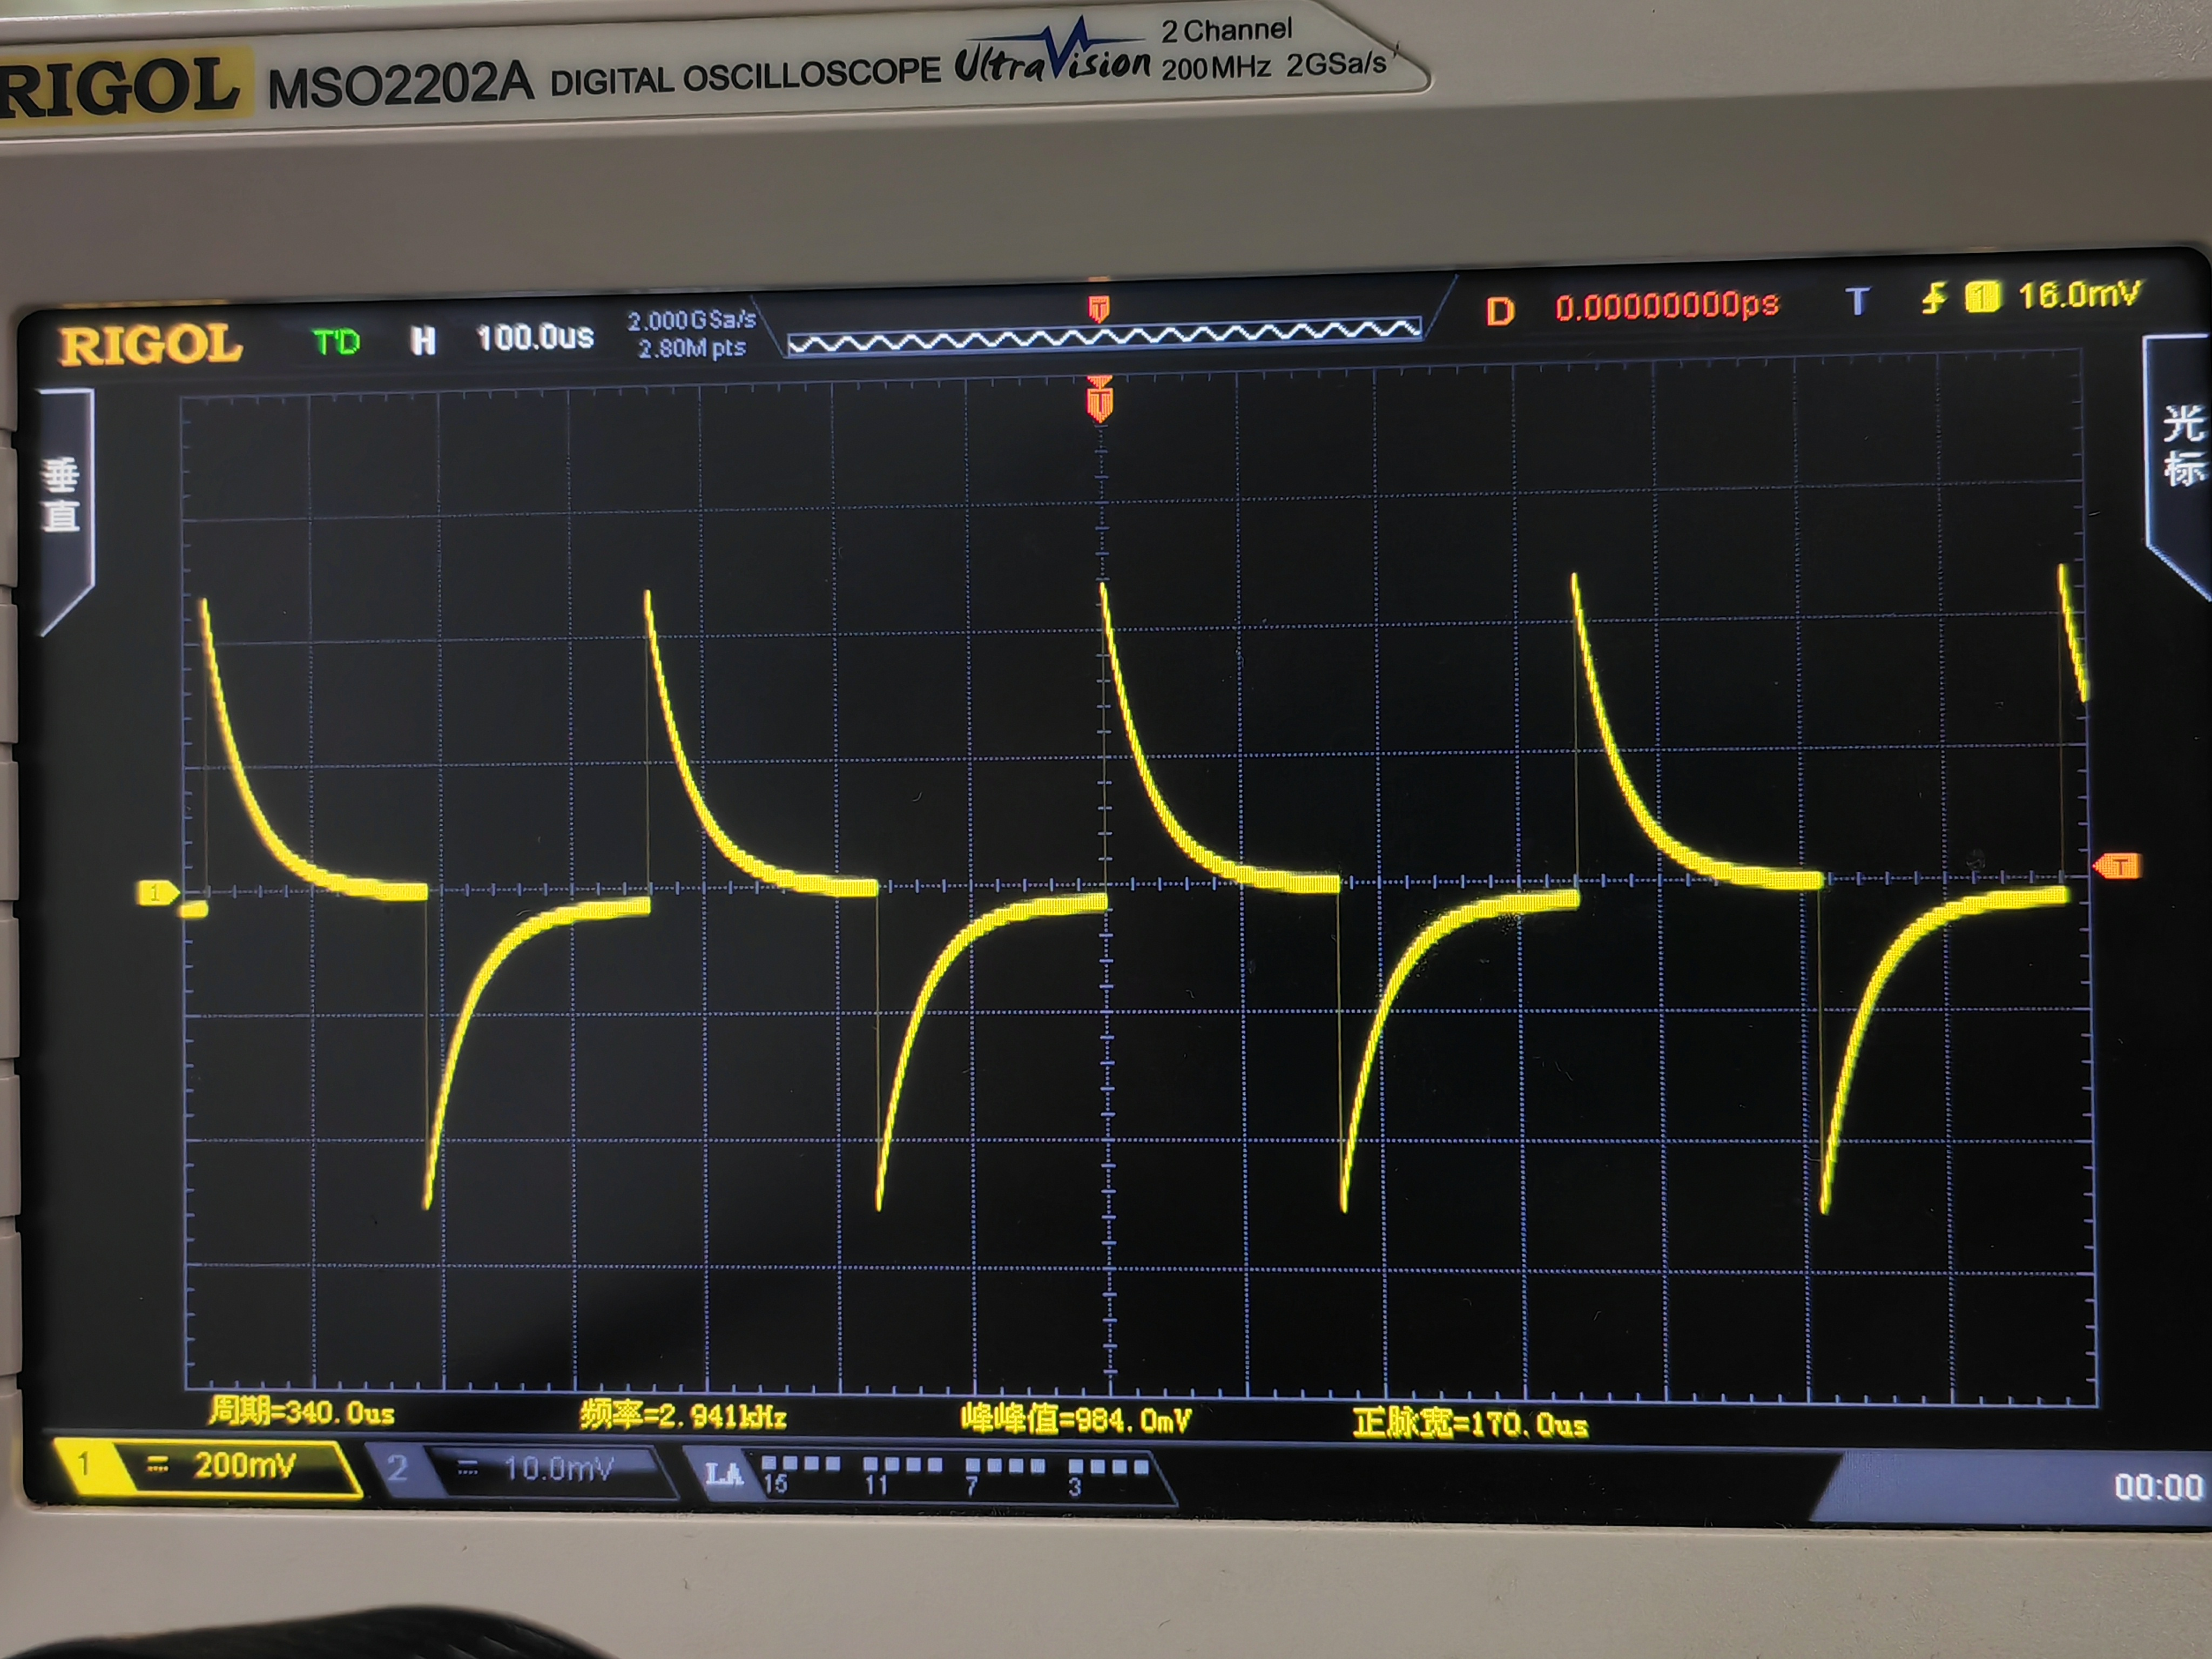
\includegraphics[width=0.35\textwidth]{2.jpg}}\hspace{6mm}
            \subfloat[时间常数测量\label{fig:3}]{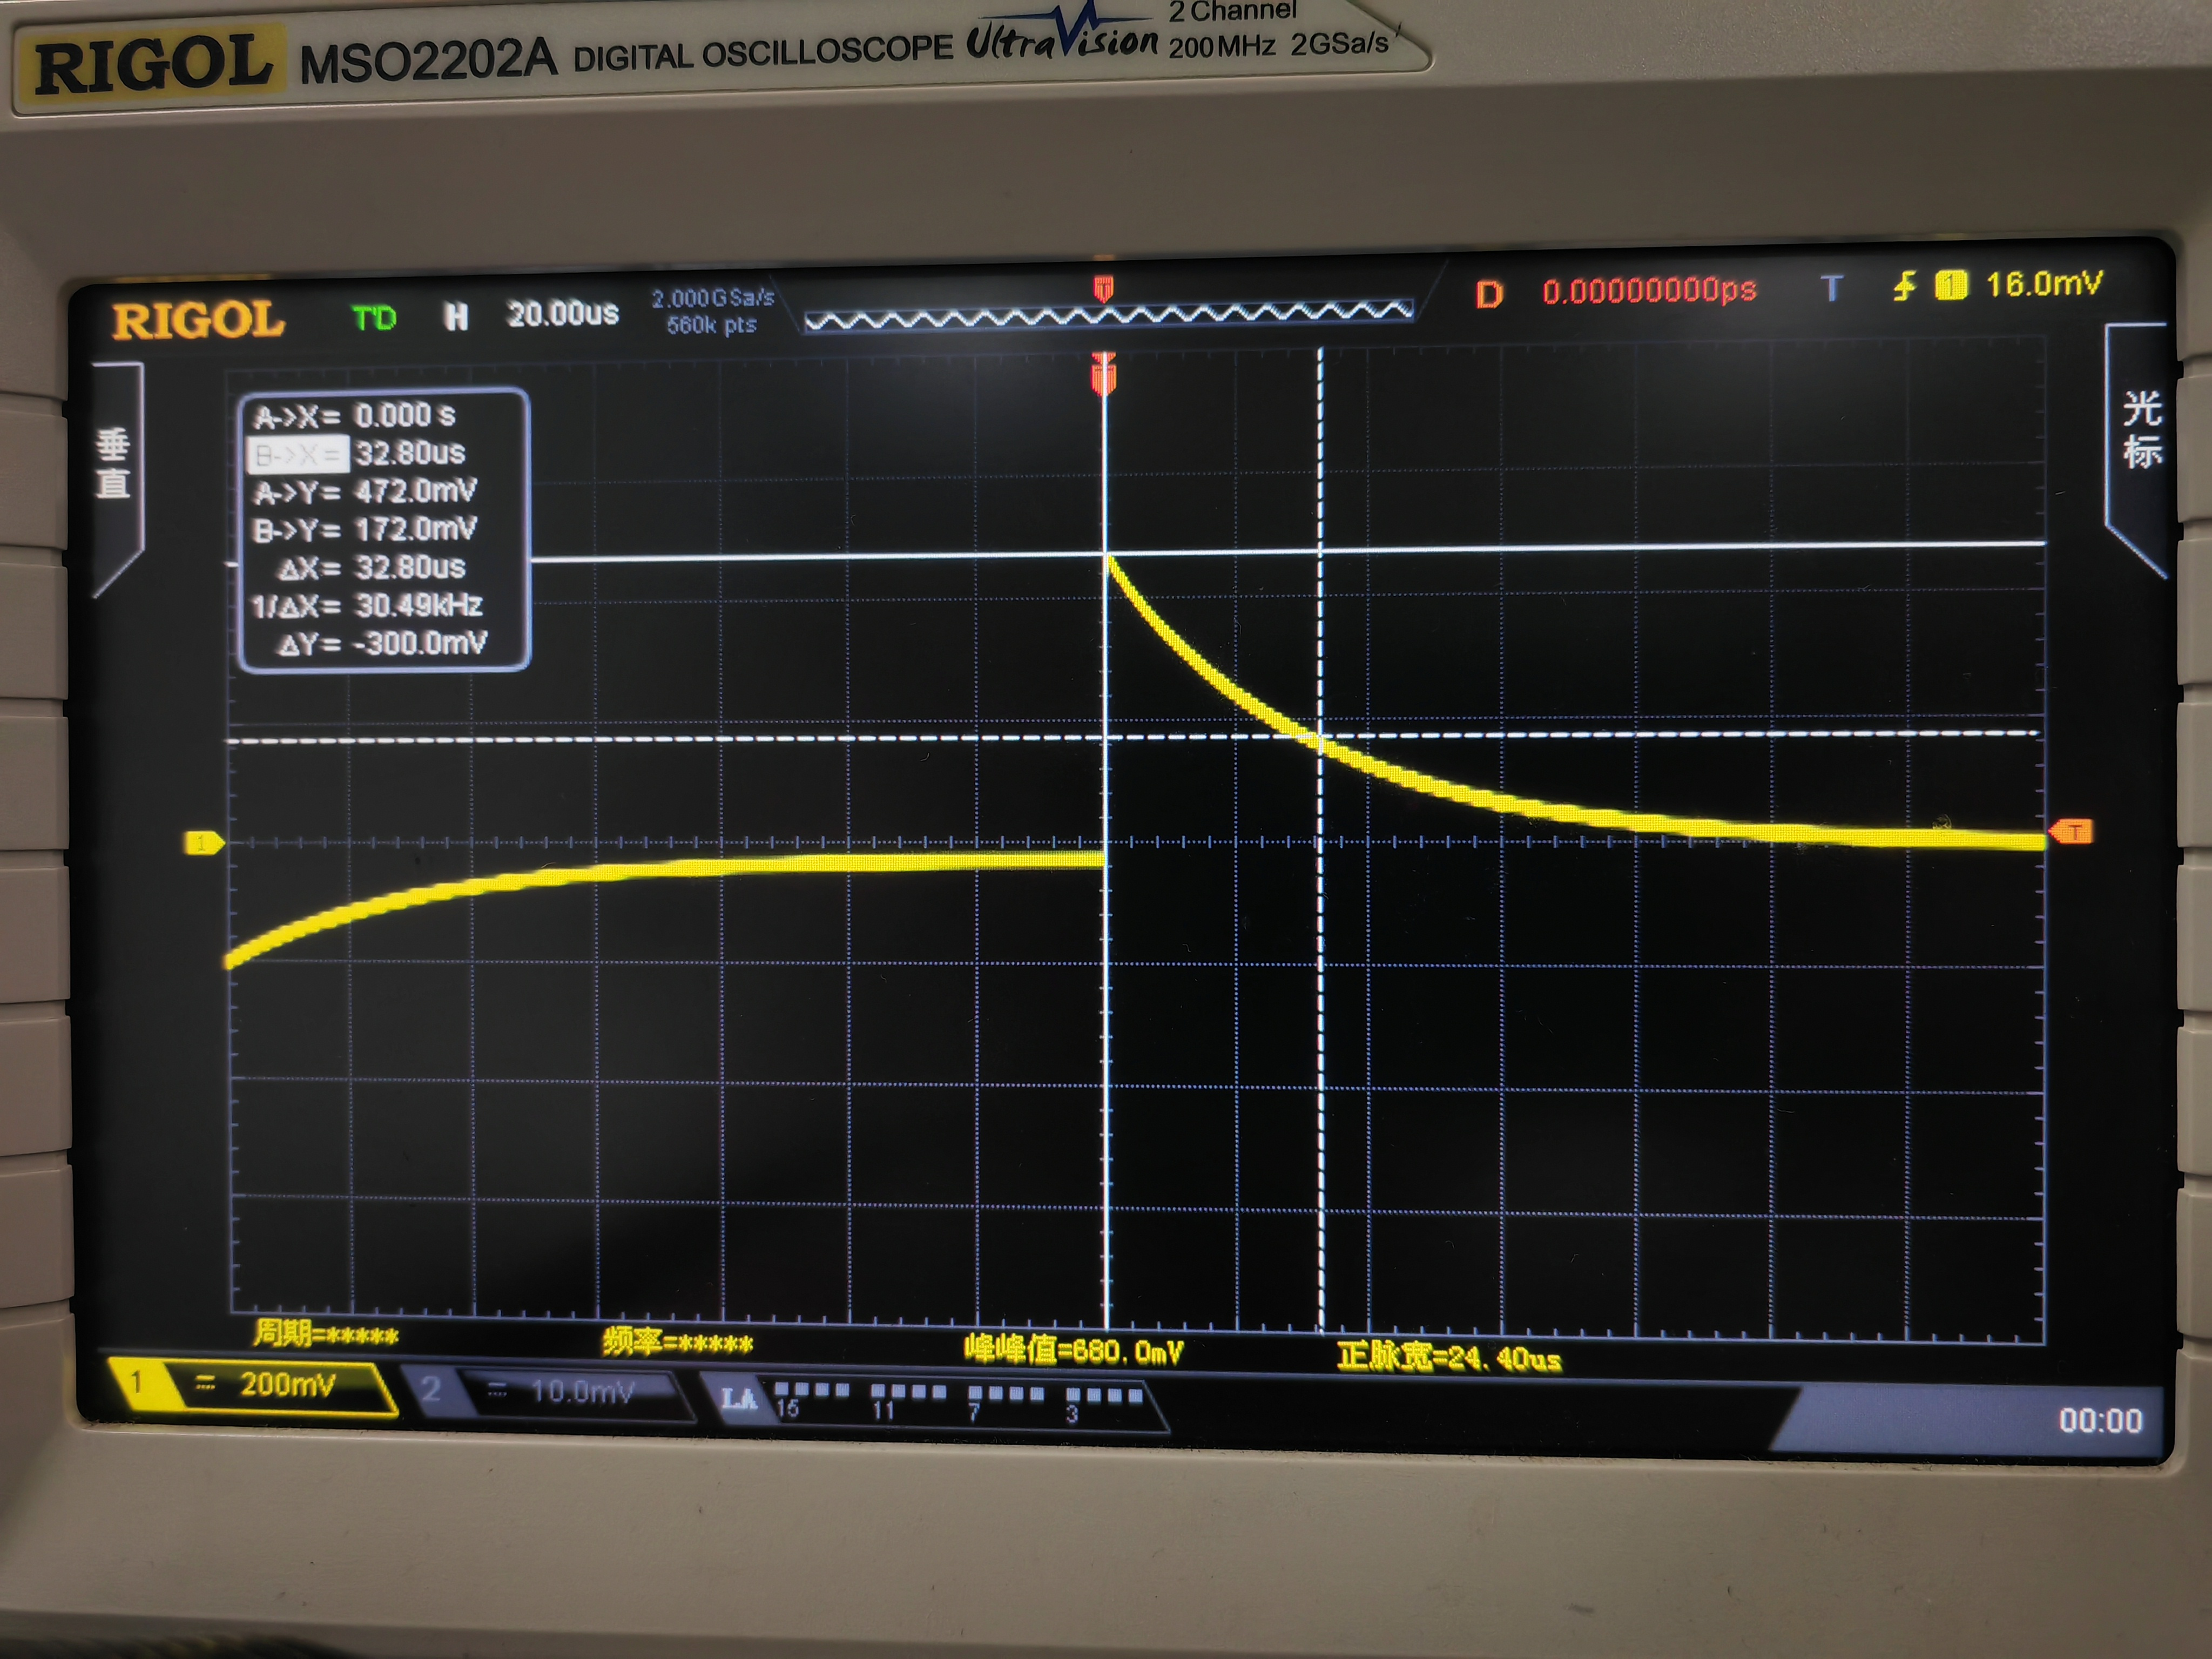
\includegraphics[width=0.35\textwidth]{3.jpg}}
            \caption{微分电路}
        \end{figure}\par
        \begin{figure}[!ht]
            \subfloat[RC积分电路图\label{fig:4a}]{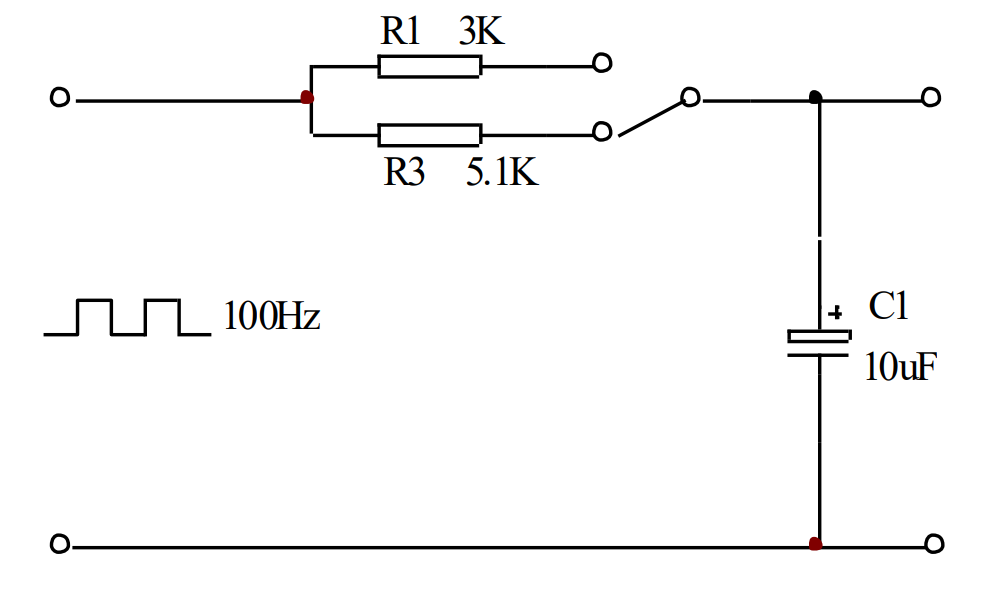
\includegraphics[width=0.35\textwidth]{4a.png}}\hspace{6mm}
            \subfloat[RL积分电路图\label{fig:4b}]{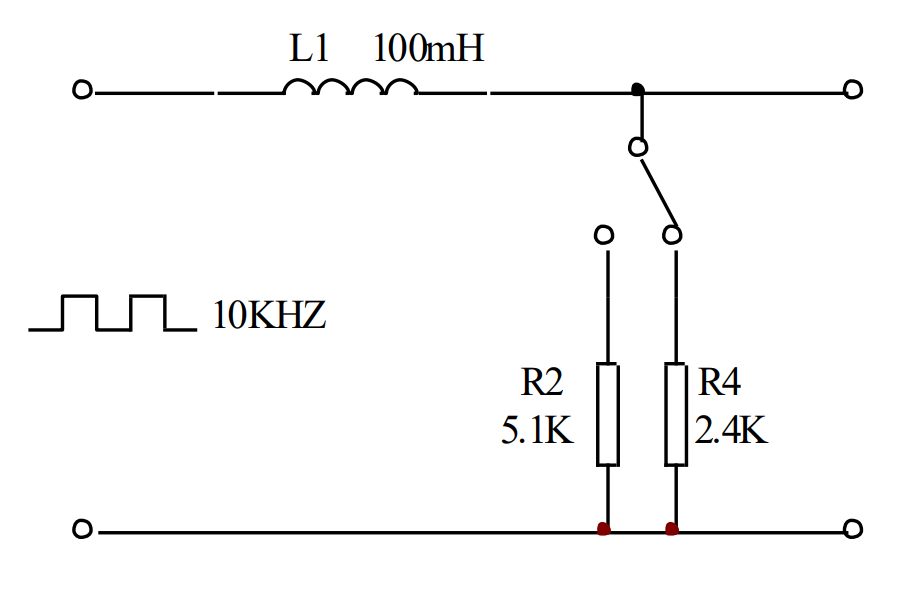
\includegraphics[width=0.35\textwidth]{4b.png}}\\
            \subfloat[电路波形\label{fig:5}]{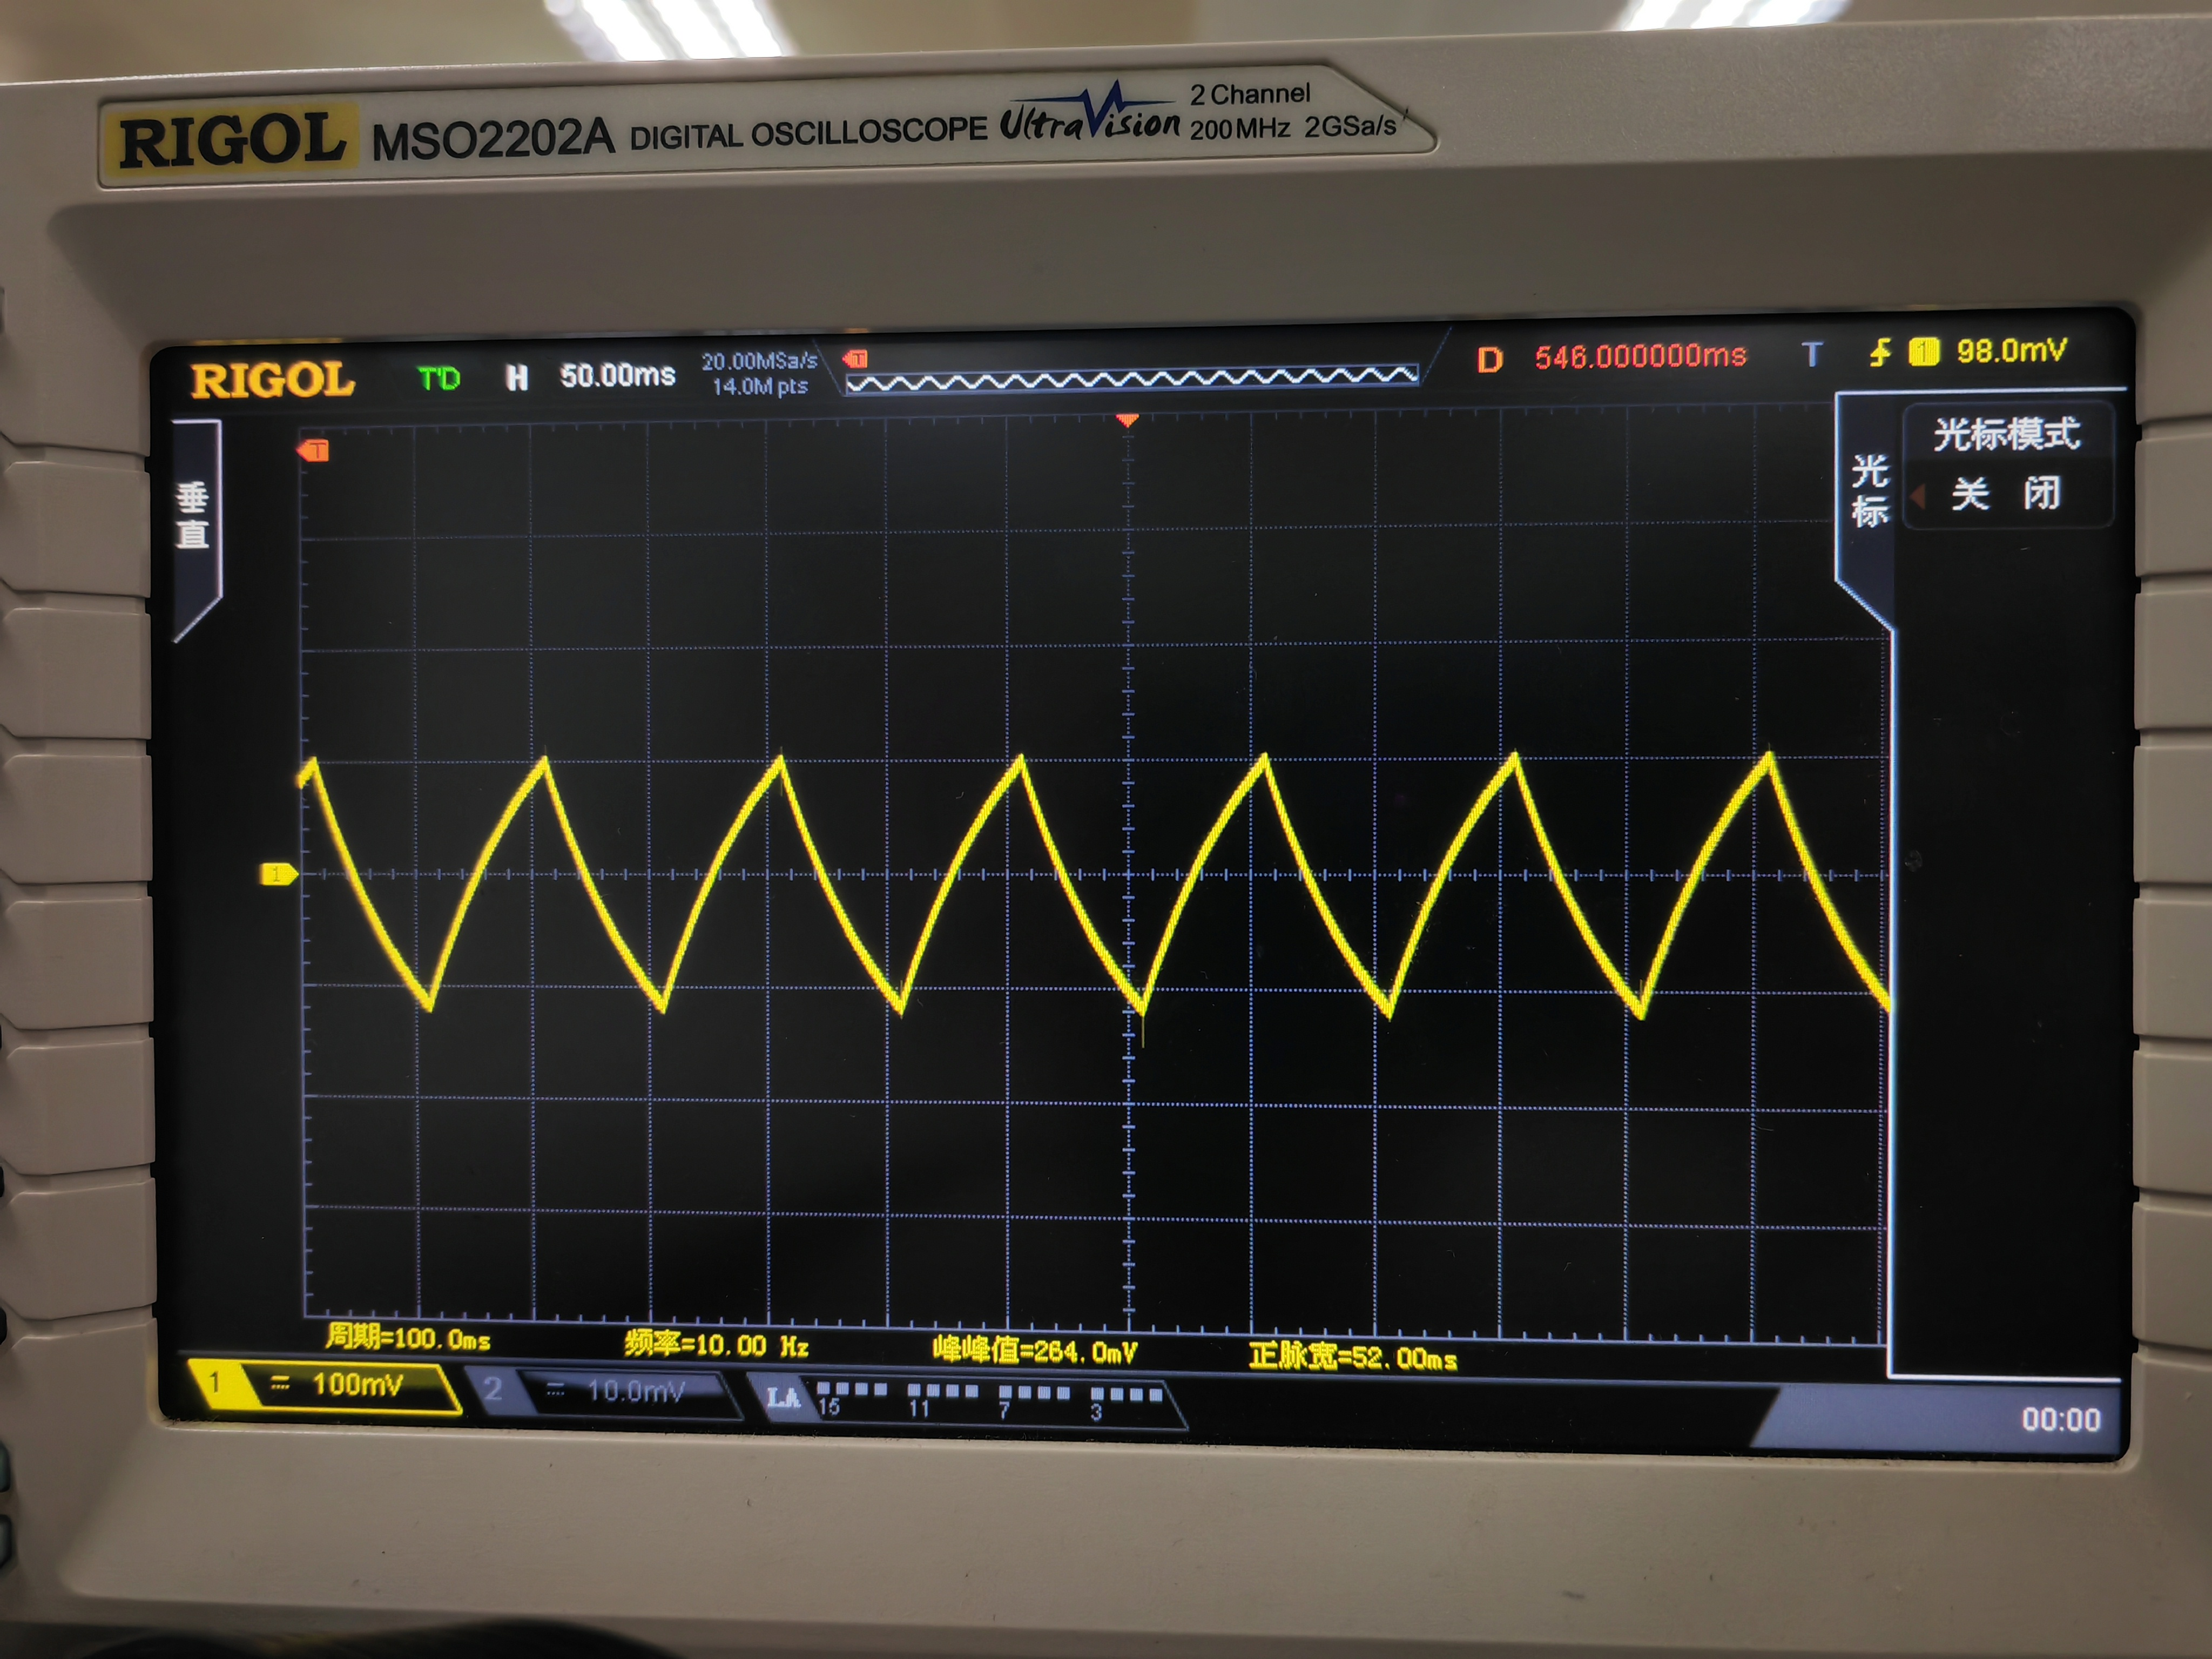
\includegraphics[width=0.35\textwidth]{5.jpg}}\hspace{6mm}
            \subfloat[时间常数测量\label{fig:6}]{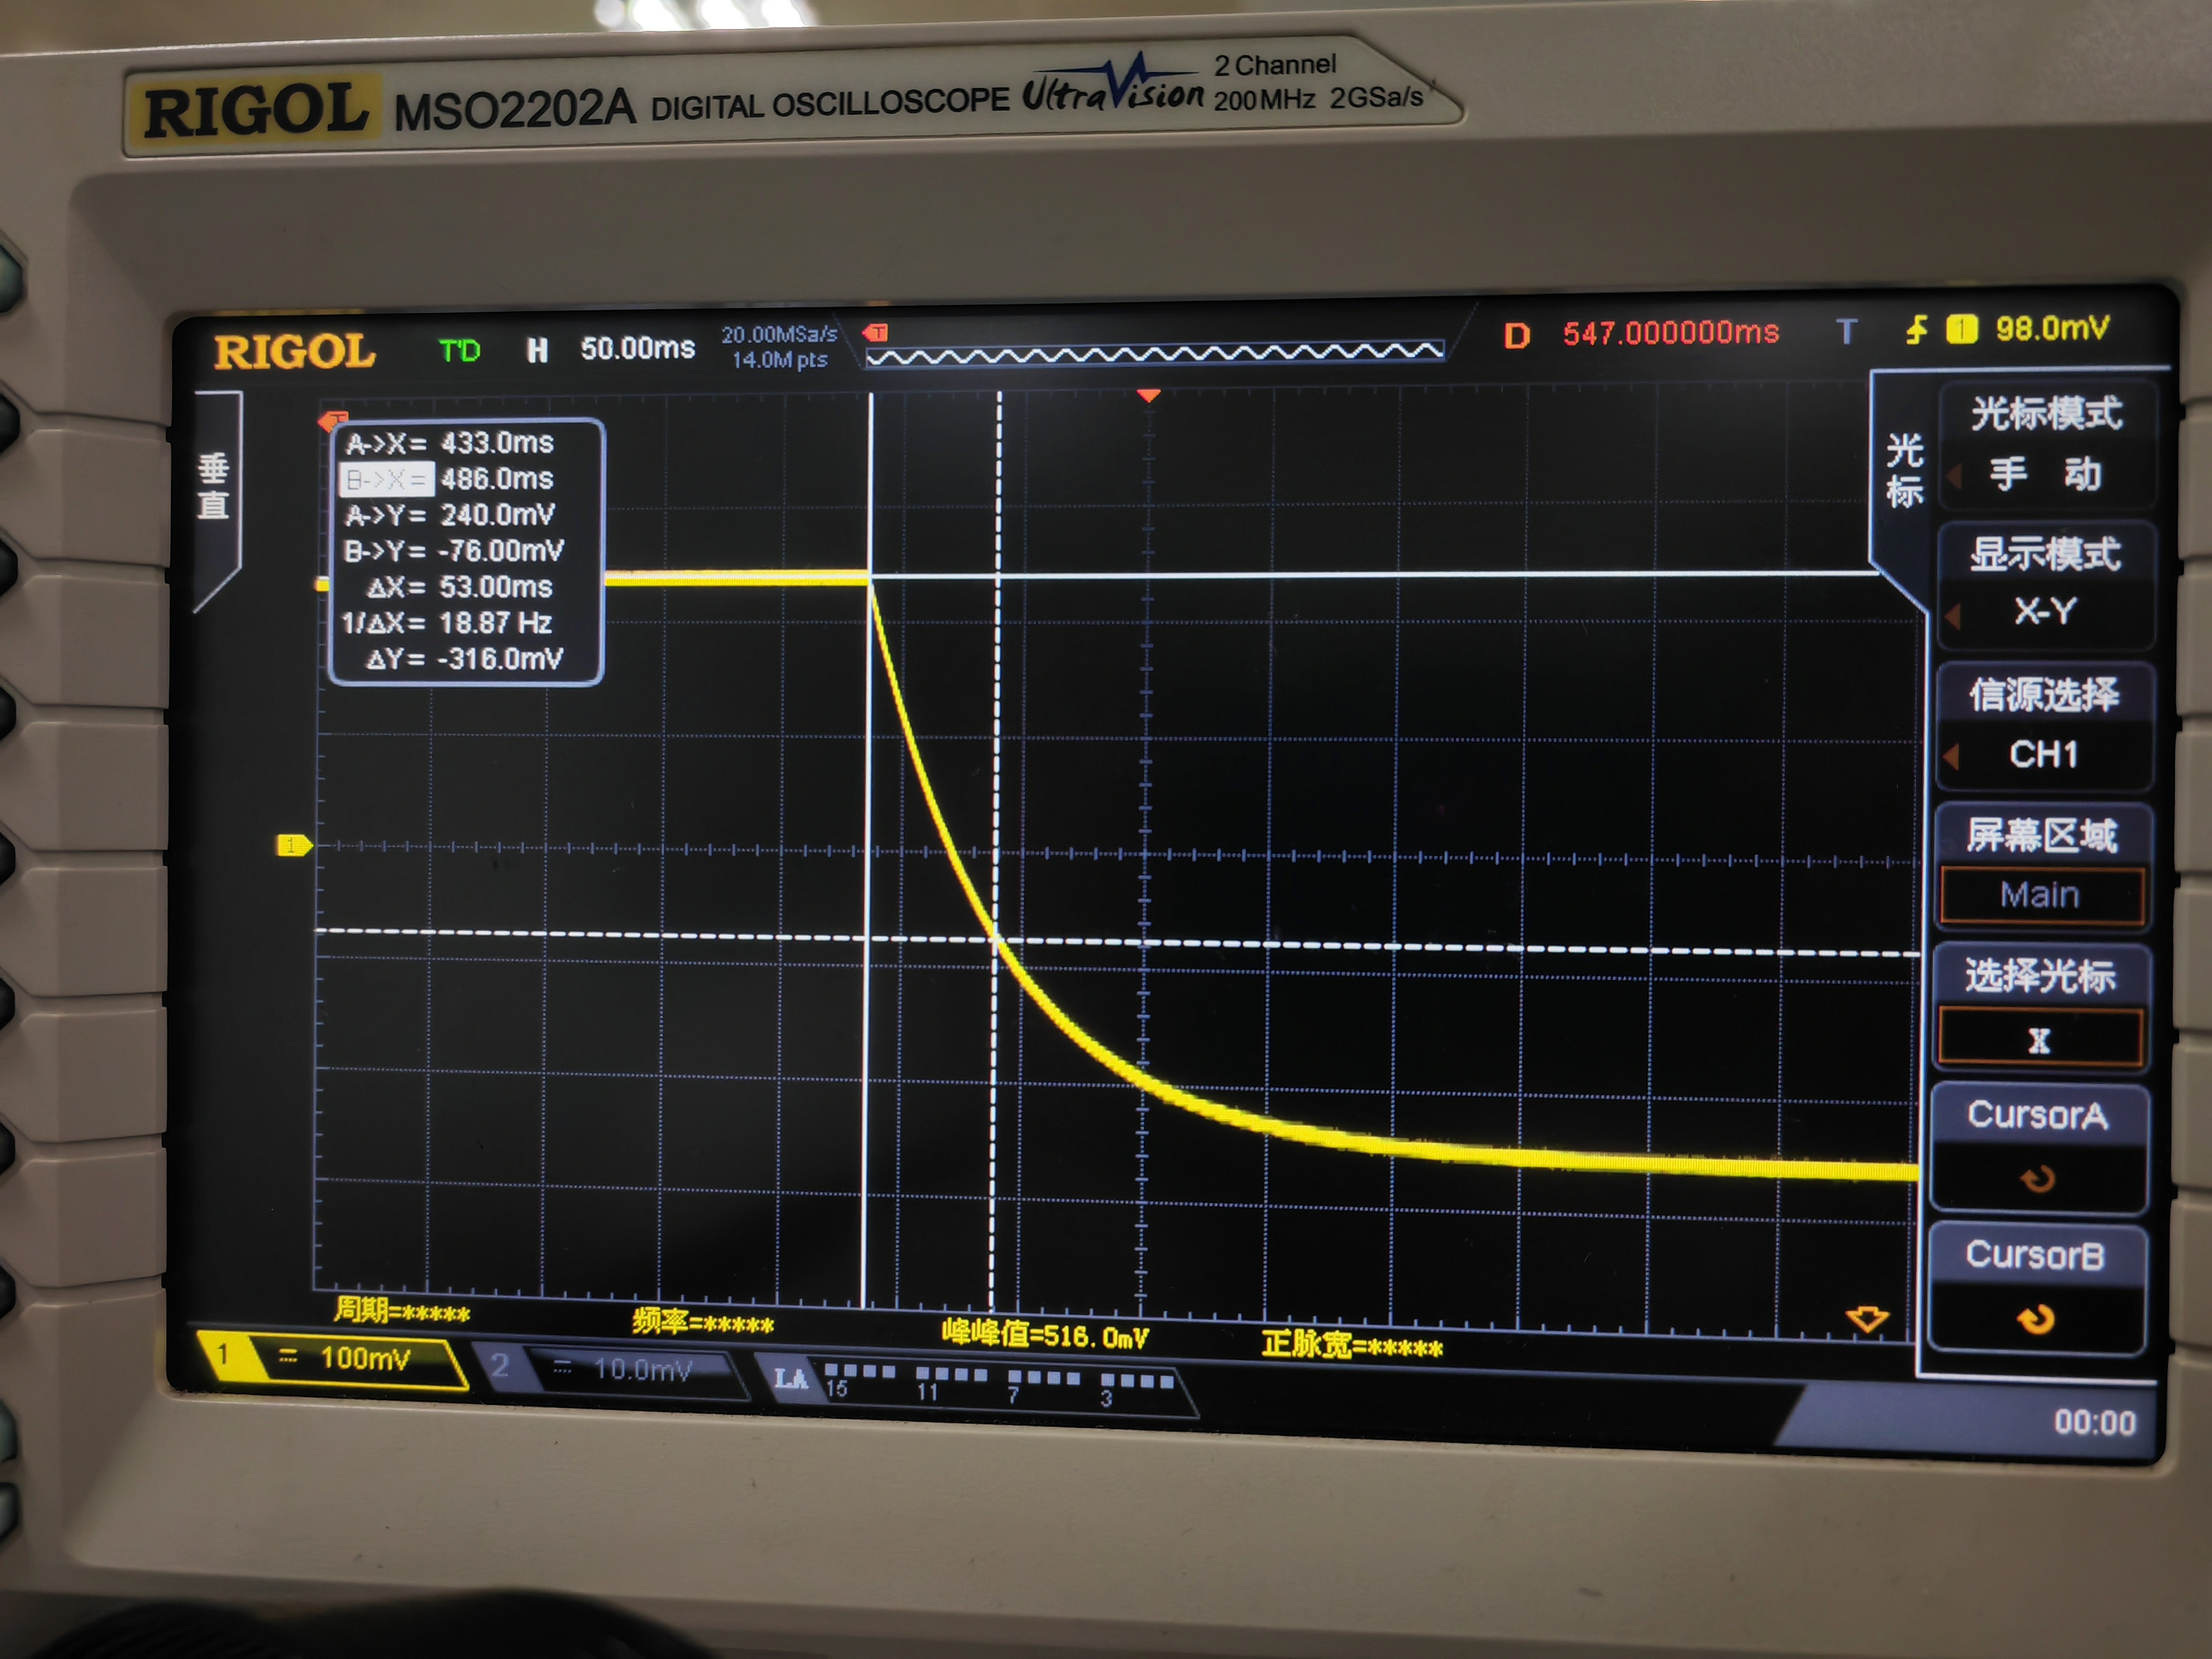
\includegraphics[width=0.35\textwidth]{6.jpg}}
            \caption{积分电路}
        \end{figure}
        \newpage
\section{实验分析}
    \subsection{分析}
    实验中根据电压下降至原先的 $\frac{1}{e}$ 所需的时间作为测量得到的时间常数 $\tau$,将其与实际计算得到的 $\tau$做对比:\par
    \begin{table}[!ht]
        \begin{tabular}{c c c}\toprule
            电路 & $\tau$计算值(\unit{\s}) & $\tau$测量值(\unit{\s}) \\ \midrule
            \multirow{2}*{RC微分电路} & $5.1*10^{-4}$& $5.2*10^{-4}$\\
             & $2.4*10^{-4}$& $2.44*10^{-4}$\\\midrule
             \multirow{2}*{RL微分电路} &$3.33*10^{-5}$& $3.28*10^{-5}$\\
             & $1.96*10^{-5}$& $1.86*10^{-5}$\\\midrule
             \multirow{2}*{RC积分电路} & $3*10^{-2}$& $3.3*10^{-2}$\\
             & $5.1*10^{-2}$ & $5.3*10^{-2}$\\\midrule
             \multirow{2}*{RL积分电路} & $1.96*10^{-5}$ & $1.96*10^{-5}$\\
             & $3.33*10^{-5}$ & $3.3*10^{-5}$\\
             \bottomrule
        \end{tabular}\caption{时间常数测量}
    \end{table}\par
    可以发现测量的结果与理论值相差很小,说明本次实验操作足够严谨,仪器使用规范。
    \subsection{误差分析}
        \begin{enumerate}
            \item 仪器输出与测量可能产生误差
            \item 线路上的电阻电感电容对结果有一定影响
        \end{enumerate}
\section{思考题}
    时间常数$\tau=RC=5.1*10^{-4}\unit{\s}$,方波脉宽应当是 $\tau$ 的20倍以上,故 $T_p \geq 1.02*10^{-2}\unit{\s}$ ,$f \leq 98\unit{\Hz}$
\section{实验心得}
    本次实验实际观察到了一阶电路的动态过程,对于动态电路又有了更加清晰明确的认知,同时也再次巩固了示波器跟函数发生器的使用。
    \clearpage
    \section{原始数据及图形}
    \begin{center}
        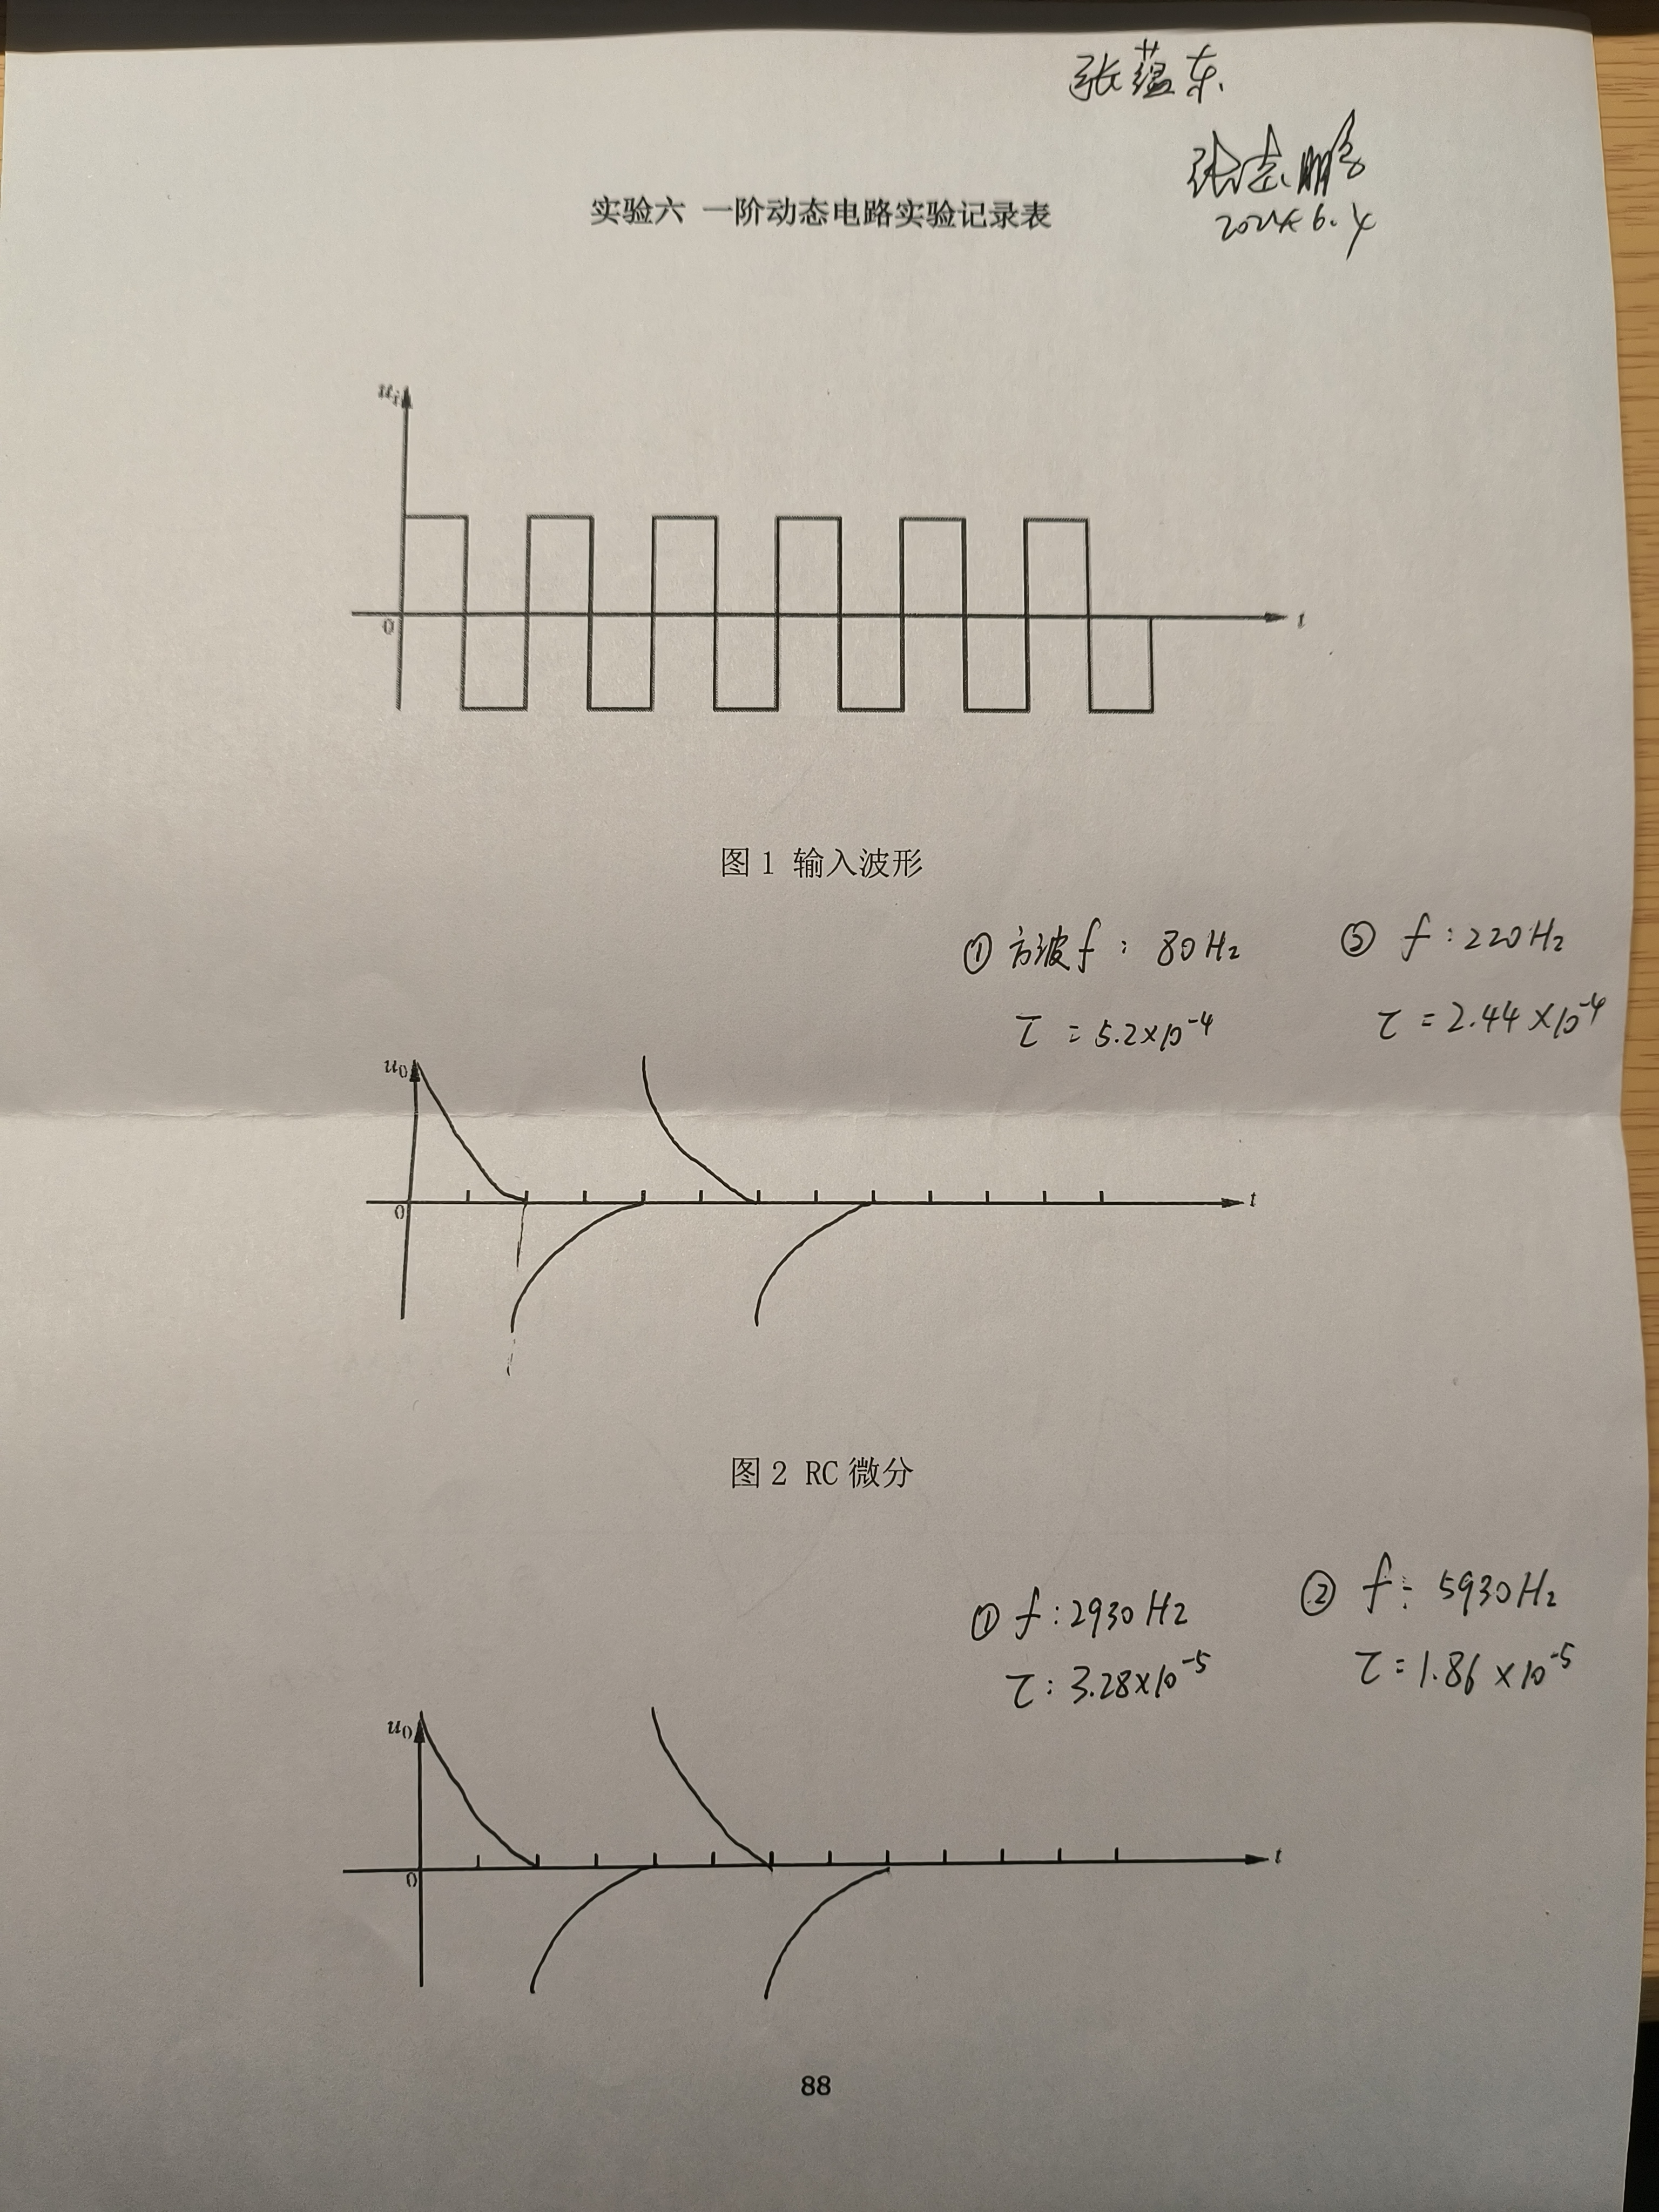
\includegraphics[width=0.7\textwidth]{7.jpg}\\
        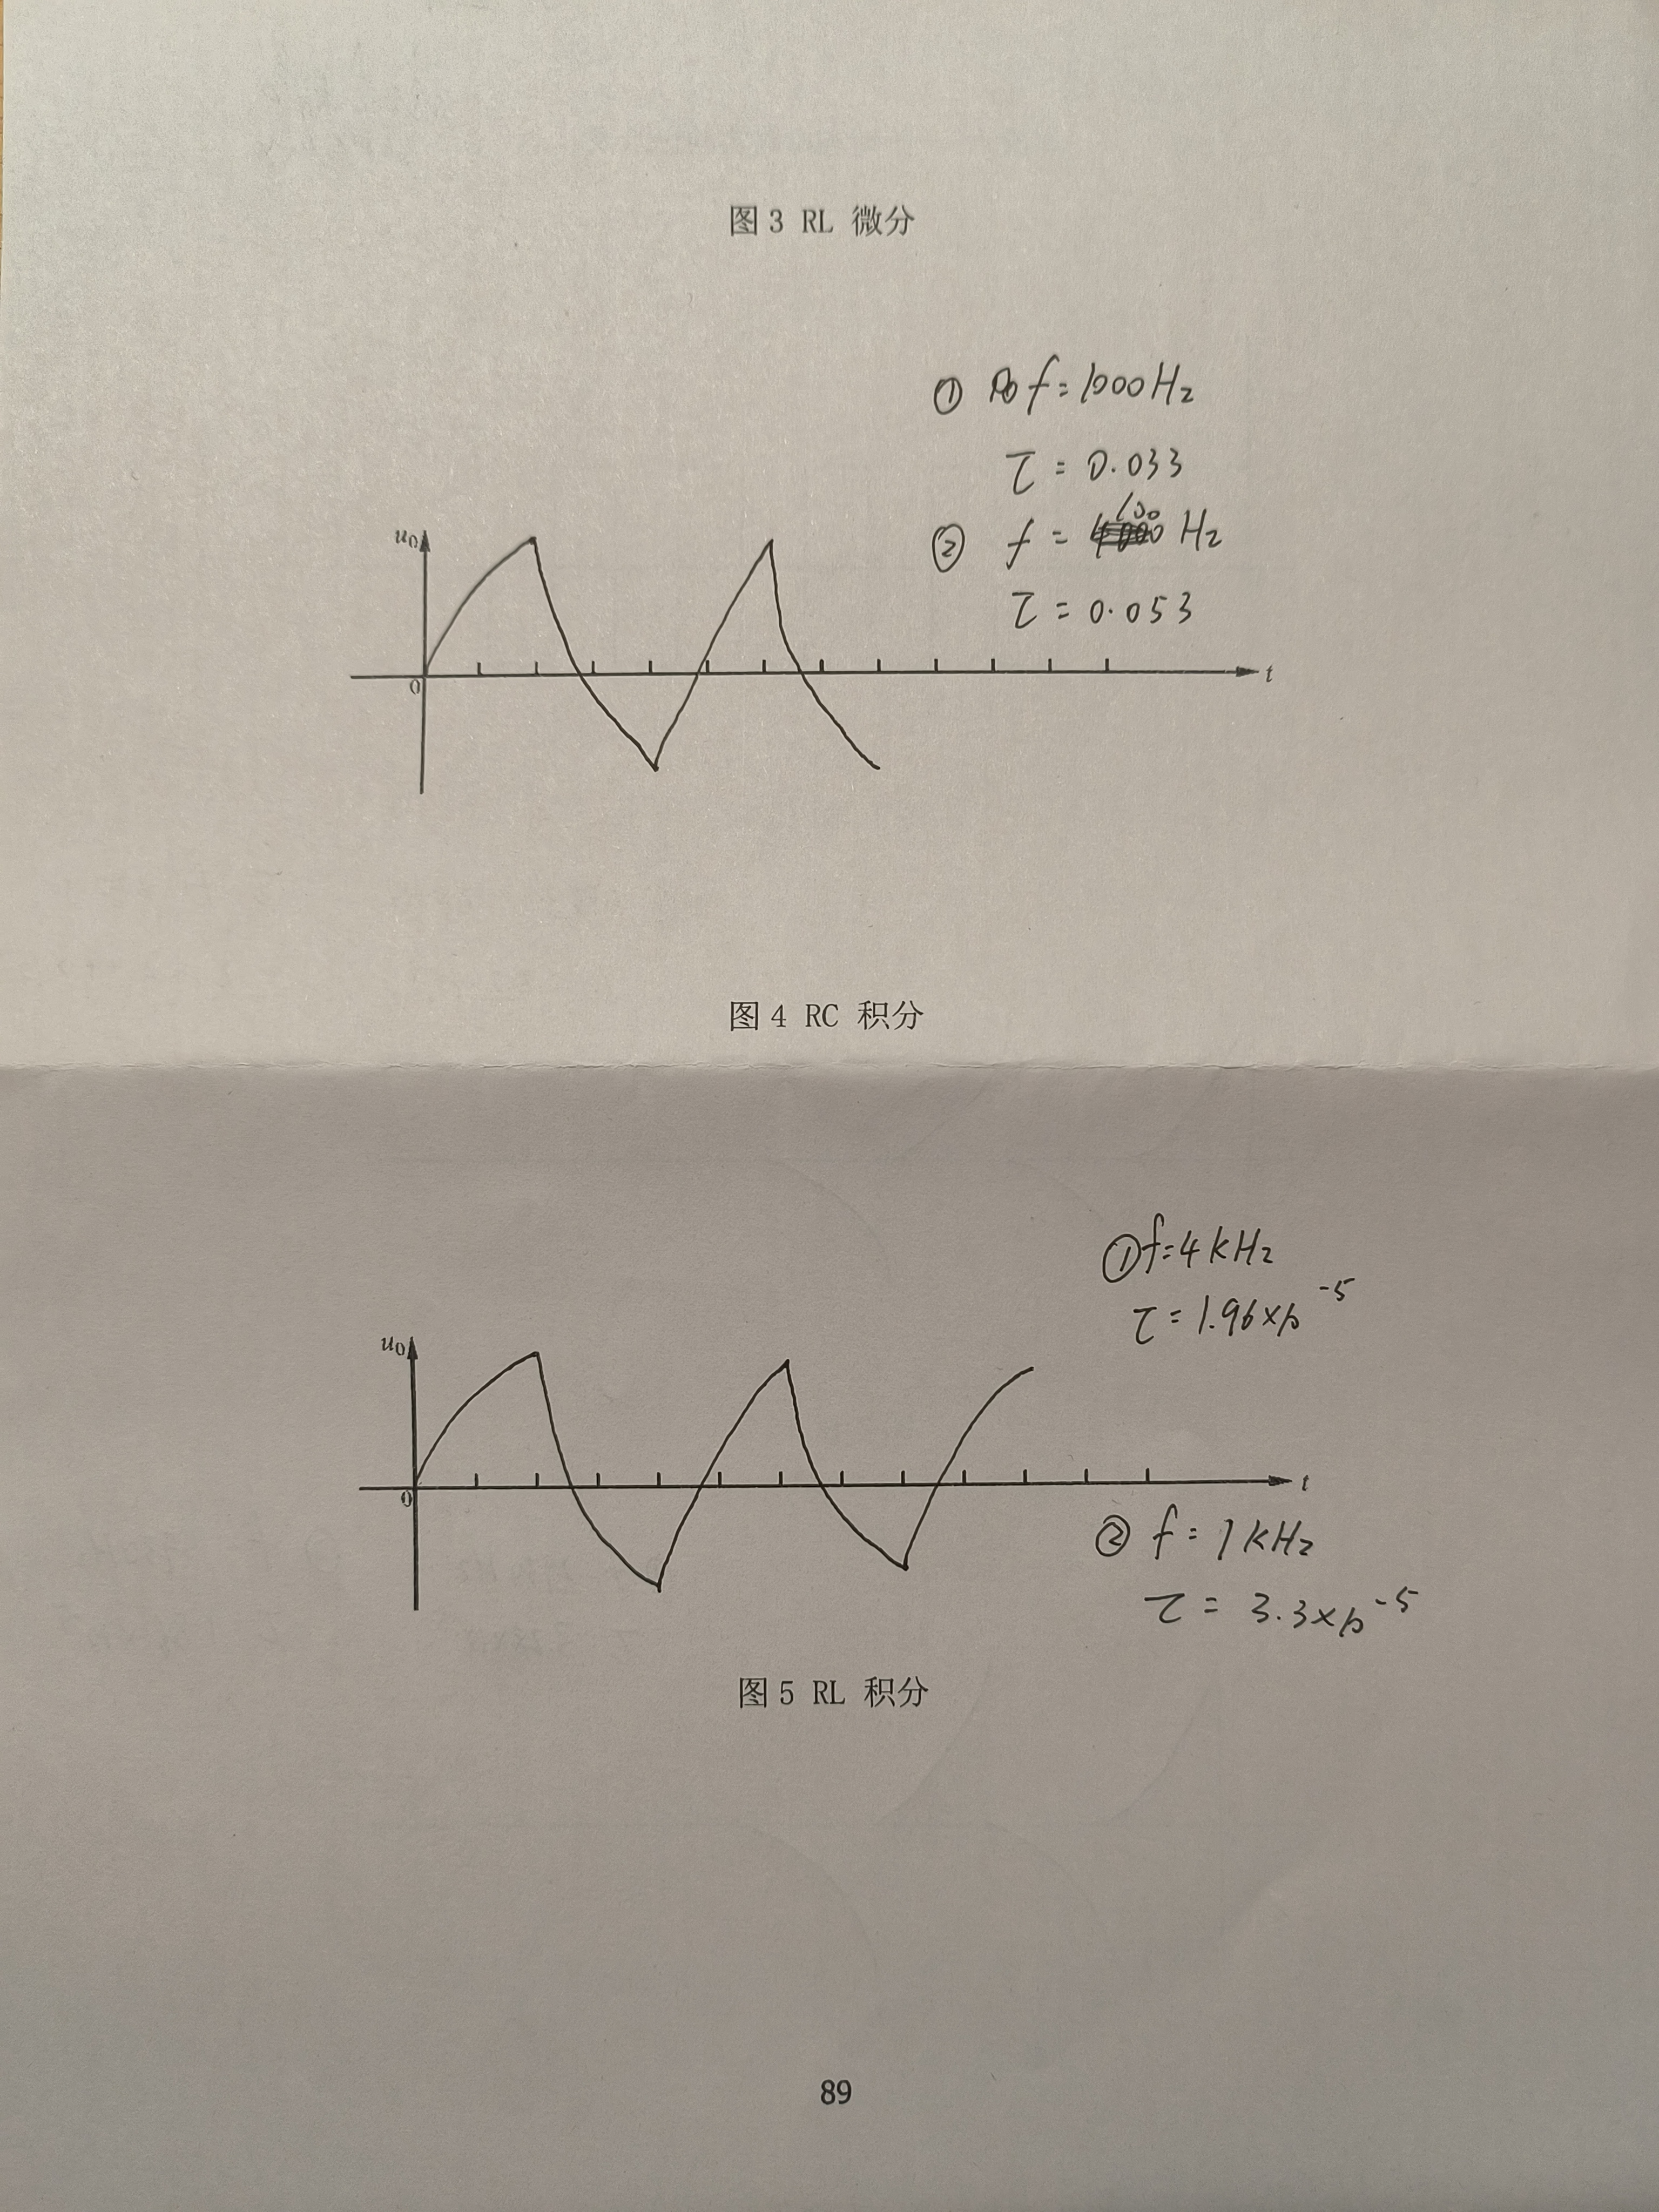
\includegraphics[width=0.7\textwidth]{8.jpg}
    \end{center}

    \end{document}